\begin{frame}[fragile]{Herzlich willkommen in der Informatik!}
	\begin{figure}[H]
		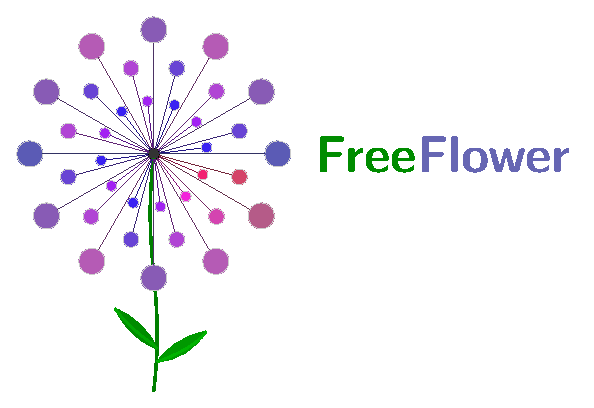
\includegraphics[width=0.8\textwidth]{Logos/FreeFlower.pdf}
	\end{figure}
\end{frame}

\begin{frame}[fragile]{Inhaltliche Ziele}
	\begin{itemize}[<+->]
		\item solide Grundlagen im Programmieren
		      \begin{itemize}[<+->]
			      \item selbstständig vollständige und korrekte Programme schreiben und verstehen
			      \item Fehler (Bugs) erkennen und beheben (Debugging)
			      \item algorithmische Ideen in Code umsetzen
			      \item Programme optimieren und erweitern
		      \end{itemize}
		\item zentrale Themen der Computerwissenschaften (nicht vollständig)
		      \begin{itemize}[<+->]
			      \item Zahlendarstellung, Kodierungen, Datentypen
			      \item Kryptographie
			      \item Algorithmen
			      \item Hardware, Funktionsweise von Computern
			      \item Kommunikation
			      \item Theoretische Informatik
			      \item Datenmanagement und Datenanalyse
			      \item Machine Learning
		      \end{itemize}
	\end{itemize}
\end{frame}

\begin{frame}[fragile]{Übergeordnete Ziele}
	\begin{itemize}[<+->]
		\item Selbstständigkeit
		\item Eigenverantwortung
		\item Frusttoleranz und eine gewisse Unbeschwertheit
		\item Computational Thinking
		\item Kollaboration
		\item formale Korrektheit und Präzision
		\item Umgang mit modernen Werkzeugen und dem eigenen Computer
	\end{itemize}
\end{frame}

\begin{frame}[fragile]{Feedback}
	\begin{itemize}
		\item Einen Grossteil der Unterlagen erstellen wir (die Fachschaft Informatik) selber.
		\item Die Unterlagen sind nicht perfekt, sondern ein laufender Prozess, der sich über die Jahre weiterentwickelt.
		\item Wir sind auf Feedback angewiesen und dankbar dafür!
		\item Wir sind sehr bemüht, Ihnen einen lehrreichen Unterricht mit zeitgemässen Inhalten zu bieten!
	\end{itemize}
\end{frame}

\begin{frame}[fragile]{Fragen stellen und Interaktion}
	\begin{itemize}
		\item Besonders in den Halbklassen habe ich viel Zeit für Sie, um Fragen zu beantworten und Ihnen zu helfen. Bitte zögern Sie nicht, Fragen zu stellen, wenn Sie etwas nicht verstehen oder wenn Sie mehr über ein Thema wissen möchten.
		\item Es ist auch wichtig, dass Sie sich aktiv am Unterricht beteiligen und mitarbeiten, damit Sie das Beste aus dem Kurs herausholen können.
		\item Ich bin wirklich sehr nett! \emoji{smile}
	\end{itemize}
\end{frame}

\begin{frame}[fragile]{Umgang mit dem Computer und Disziplin}
	\begin{itemize}
		\item Elektronische Geräte bieten viele Möglichkeiten, aber auch viele Ablenkungen. Es ist wichtig, dass Sie lernen, damit umzugehen.
		\item Ich werde Sie immer mal wieder bitten, die Laptops zu schliessen, damit wir uns auf die Inhalte konzentrieren können.
	\end{itemize}
\end{frame}

\begin{frame}[fragile]{Niveau}
	\begin{mycaution}
		Wir haben hohe Ansprüche an Sie und das Niveau ist hoch (i.e. Gymi-Level). Nehmen Sie die Inhalte und die Prüfungen ernst.
	\end{mycaution}
\end{frame}

\begin{frame}[fragile]{Unterlagen}
	\url{https://moodle.ksimlee.ch/}
\end{frame}
